\section{Methodology}
\begin{figure}[!htbp]
\centering
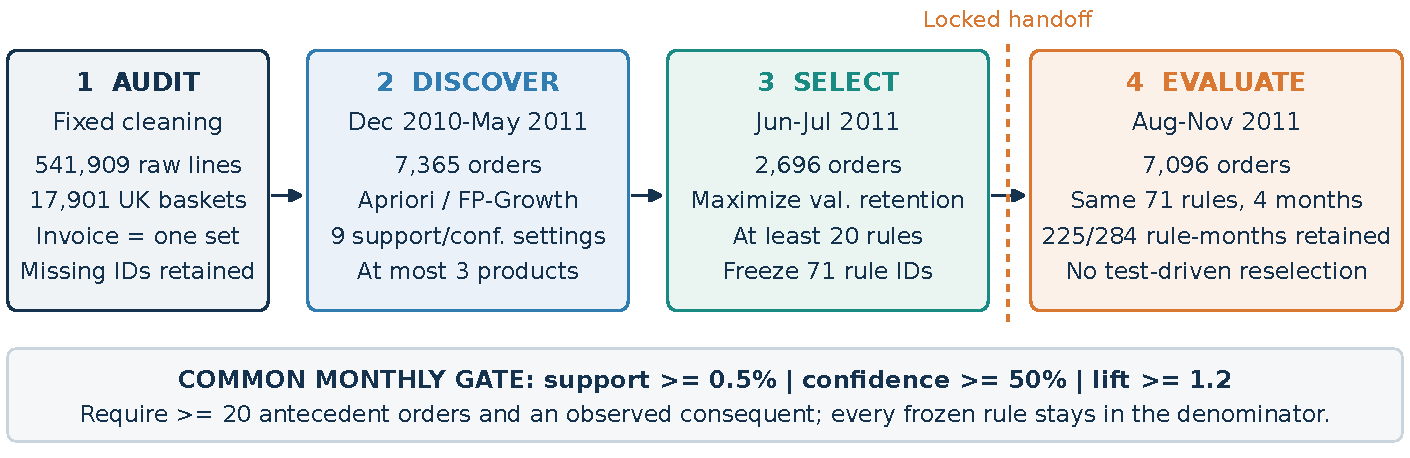
\includegraphics[width=\linewidth]{08_method_overview.pdf}
\caption{\textbf{Temporal evaluation overview.} Validation selects a discovery cohort before test evaluation. The dashed line marks frozen rule IDs and parameters. Every rule remains in each test month's denominator, including those with insufficient evidence. Diagnostics do not change the primary selection.}
\label{fig:overview}
\end{figure}

\subsection{Audited invoice-level observations}
Sequential cleaning reduces \RawRows{} raw lines to \CleanRows{} positive-sales lines and \AllOrders{} baskets across all countries; \UKOrders{} UK baskets define the primary population. Exact duplicates, cancellations, nonpositive quantities/prices and explicit non-product codes are excluded. The full reconciliation is in Appendix~\ref{app:audit}. Original purchases are not matched against later returns, so baskets do not represent net fulfilled sales.

The \MissingCustomers{} rows without a customer ID (\MissingCustomerPct{}) remain eligible: invoice number, product code and date suffice for this task. Codes define product identity; descriptions provide labels only. Valid alphanumeric codes and singleton baskets remain. For 42 invoices whose two timestamps differ by one minute on the same day, we use the earliest timestamp. Cross-day or cross-country invoice conflicts would halt processing.

\subsection{Equivalent bounded discovery}
Discovery orders are encoded as a Boolean matrix. Singleton products below the lowest discovery support are removed using discovery data only; downward closure makes this pruning lossless for the bounded search. An order emptied by pruning remains an all-false row, preserving support denominators.

Apriori searches candidates level by level, whereas FP-Growth uses compressed prefix trees~\citep{agrawal1994,han2000}. Both MLxtend implementations~\citep{raschka2018} receive the same matrix, support thresholds and maximum itemset length of three; Apriori uses its low-memory mode. We generate single-consequent rules, then filter discovery confidence and lift. Canonical signatures of sorted itemsets and integer counts test exact output equivalence.

For a frequent three-product itemset, each allowed rule has one consequent and the other two products as its antecedent. Keeping this representation identical prevents changes in rule construction from being mistaken for differences between mining algorithms.

\subsection{Selection and evaluation boundary}
Validation maximizes mean retention subject to at least 20 rules, with fixed tie-breaks given in Section~\ref{sec:settings}. Source and configuration checksums are recorded before evaluation; selected parameters and the rule-ID hash are saved before test metrics. Monthly basket counts evaluate every frozen rule without re-discovery. Independent direct scans verify sampled counts; rolling cohorts remain separate comparisons.

